% TI Agent: project report
% Build:  latexmk -pdf main.tex        (pdflatex + biber; output main.pdf)
% Screenshots: drop the PNG files listed in figures/README.txt into figures/. Until a file is
% there, the PDF shows a labelled placeholder box in its place.

\documentclass[11pt,a4paper]{article}

% ------------------------------------------------------------------ packages
\usepackage[T1]{fontenc}
\usepackage[utf8]{inputenc}
\usepackage{lmodern}
\usepackage{microtype}
\usepackage[margin=2.5cm]{geometry}
\usepackage{graphicx}
\usepackage{xcolor}
\usepackage{booktabs}
\usepackage{tabularx}
\usepackage{array}
\usepackage{amsmath}
\usepackage{enumitem}
\usepackage{caption}
\usepackage{float}
\usepackage{listings}
\usepackage{tikz}
\usetikzlibrary{positioning, arrows.meta, shapes.geometric, fit, backgrounds, calc}
\usepackage{pgfplots}
\pgfplotsset{compat=1.18}
\usepackage[backend=biber, style=numeric, sorting=none, maxbibnames=4]{biblatex}
\addbibresource{references.bib}
\usepackage[colorlinks=true, linkcolor=accent, citecolor=accent, urlcolor=accent]{hyperref}

% ------------------------------------------------------------------ look
\definecolor{accent}{HTML}{1F5FA8}
\definecolor{ink}{HTML}{22262B}
\definecolor{muted}{HTML}{6B7280}
\definecolor{boxfill}{HTML}{EEF3FA}
\definecolor{storefill}{HTML}{E8F3EC}
\definecolor{extfill}{HTML}{F5F1E8}
\definecolor{warnfill}{HTML}{FBEDEA}
\definecolor{good}{HTML}{2E7D4F}
\definecolor{bad}{HTML}{B23B3B}
\definecolor{neutral}{HTML}{8A8F98}

\setlist{itemsep=2pt, topsep=4pt}
\captionsetup{font=small, labelfont=bf}
\renewcommand{\arraystretch}{1.15}
\lstset{basicstyle=\ttfamily\footnotesize, columns=flexible, keepspaces=true, showstringspaces=false,
        frame=single, rulecolor=\color{muted!40}, backgroundcolor=\color{boxfill!40},
        xleftmargin=4pt, xrightmargin=4pt, breaklines=false}

\tikzset{
  % no hyphenation inside diagram boxes: words wrap whole
  block/.style   = {draw=accent!70, fill=boxfill, rounded corners=2pt, align=center,
                    font=\small, minimum height=8mm, inner sep=4pt, text width=#1,
                    execute at begin node={\hyphenpenalty=10000\exhyphenpenalty=10000}},
  block/.default = 2.6cm,
  ext/.style     = {draw=muted!70, fill=extfill, rounded corners=2pt, align=center,
                    font=\small, minimum height=7mm, inner sep=3pt, text width=#1,
                    execute at begin node={\hyphenpenalty=10000\exhyphenpenalty=10000}},
  ext/.default   = 2.4cm,
  store/.style   = {cylinder, shape border rotate=90, aspect=0.22, draw=good!70, fill=storefill,
                    align=center, font=\small, minimum height=14mm, text width=#1},
  store/.default = 2.8cm,
  arr/.style     = {-{Stealth[length=2.2mm]}, thick, draw=ink!70},
  dasharr/.style = {-{Stealth[length=2.2mm]}, thick, dashed, draw=muted},
  lbl/.style     = {font=\scriptsize, text=muted, align=center},
  group/.style   = {draw=muted!50, dashed, rounded corners=4pt, inner sep=6pt},
}

% A screenshot if the file is in figures/, otherwise a labelled placeholder.
\newcommand{\screenshot}[4][0.85]{%
  \begin{figure}[htbp]
    \centering
    \IfFileExists{figures/#2}%
      {\includegraphics[width=#1\linewidth]{figures/#2}}%
      {\fcolorbox{muted!60}{boxfill!35}{\parbox[c][4.2cm][c]{#1\linewidth}{\centering\small\sffamily\color{muted}%
        Screenshot placeholder\\[2pt]\texttt{figures/#2}}}}
    \caption{#3}\label{#4}
  \end{figure}}

\newcommand{\code}[1]{\texttt{#1}}

\title{\textbf{TI Agent}\\[4pt]\large A local, cited AI research assistant for US equities:\\how it was built, what it does, and what broke along the way}
\author{Nanda Srikanth Saroj Kumar Nanda}
\date{14 November 2026}

\begin{document}
\maketitle

\begin{abstract}
TI Agent screens about 900 large- and mid-cap US stocks every week, keeps the twenty most promising,
and asks a small local language model to write a medium-term and a long-term view of each one. Every
claim in those views has to point at a passage the model actually retrieved, and every number has to
match a value that code computed. The whole system runs on one laptop with free data sources: a local
PostgreSQL database with vector search, a 4-billion-parameter model in Ollama, and Windows scheduled
tasks. Results reach readers through a Flutter app on GitHub Pages that downloads a single
password-encrypted file and decrypts it in the browser, so nothing needs to run online. This report
walks through the design phase by phase, explains the choices behind it, and documents the first full
run on the local database, including the memory problems it ran into and how they were fixed.
\end{abstract}

\begin{center}
\fcolorbox{bad!50}{warnfill}{\parbox{0.9\linewidth}{\small\textbf{Disclaimer.} TI Agent is a research and
learning project. Nothing it produces is financial advice, and it never places trades.}}
\end{center}

\tableofcontents
\newpage

% ==================================================================
\section{Why I built it}

Most of what an analyst does before forming a view on a stock is reading: filings, news, the numbers
behind the price chart. Large language models are good at reading, but they have two habits that make
them dangerous in finance. They state numbers with confidence whether or not the numbers are real, and
they quietly use what they memorised during training, which in a backtest means using the future.

I wanted to see how far a small, free, local model could go if the surrounding system took those habits
away. That became four rules that shaped almost every later decision:

\begin{enumerate}
  \item \textbf{No lookahead.} Everything the model sees must have been public before the date it is
        reasoning about.
  \item \textbf{Numbers come from code.} The model may only repeat figures that a tool computed.
  \item \textbf{Every claim is cited.} A view is saved only if its sources were really retrieved in the
        same conversation.
  \item \textbf{Free and local.} Free data, a model that runs on a laptop GPU, no paid services.
\end{enumerate}

The project is organised into ten modules (M1 to M10) and five phases. Each phase ends with a
\emph{gate}, a measurable condition that has to hold before the next phase builds on it.
Table~\ref{tab:phases} gives the overview; the rest of the report follows the same order.

\begin{table}[htbp]
\centering\small
\begin{tabularx}{\linewidth}{@{}l X X l@{}}
\toprule
Phase & What it delivers & Gate & Status \\
\midrule
P1 Foundations & Point-in-time data, collected daily and stored locally & 7 clean daily runs & Restarted on the local database \\
P2 Knowledge   & Computed features and hybrid search & Relevant passages for 10 test queries & Passed (10/10) \\
Screen         & The 20 picks from about 900 stocks & --- & Running weekly \\
P3 Agent       & Weekly cited views and a Telegram digest & 4 valid, cited weekly runs & 1 of 4 \\
P4 App         & Flutter app on GitHub Pages and Android & Testers use it for 2 weeks & Live \\
P5 Evaluation  & Scoring views against outcomes and baselines & 12 closed weeks & Built, 0 of 12 \\
P5 Quantum     & Quantum vs classical portfolios & Benchmark report & Not started \\
\bottomrule
\end{tabularx}
\caption{Phases, their gates and where each one stands on 14 November 2026.}
\label{tab:phases}
\end{table}

% ==================================================================
\section{The system at a glance}

Figure~\ref{fig:arch} shows the moving parts. Data comes in from five free sources, is cleaned and
indexed into one database, and is read back by the quant engine, the search layer and the agent. The
database is the only connection between modules: nothing calls another module directly, and every read
and write goes through one small store class. That single seam is also what made the later move from a
hosted database to a local one cheap, and it lets the 130 offline tests swap the database for an
in-memory fake.

\begin{figure}[htbp]
\centering
\resizebox{\linewidth}{!}{%
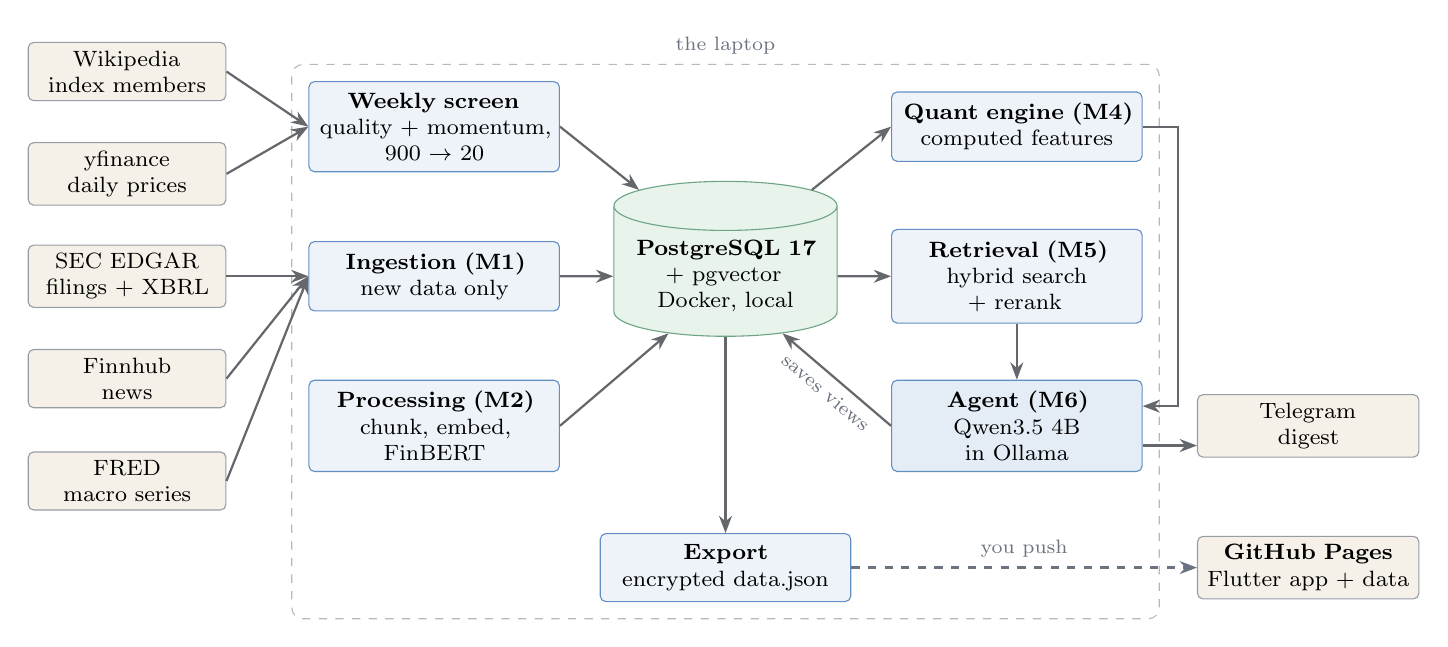
\begin{tikzpicture}[block/.append style={font=\footnotesize}, ext/.append style={font=\footnotesize},
                    store/.append style={font=\footnotesize}]
  % sources
  \node[ext=2.3cm] (wiki) at (0, 2.6)  {Wikipedia\\index members};
  \node[ext=2.3cm] (yf)   at (0, 1.3)  {yfinance\\daily prices};
  \node[ext=2.3cm] (sec)  at (0, 0)    {SEC EDGAR\\filings + XBRL};
  \node[ext=2.3cm] (fin)  at (0, -1.3) {Finnhub\\news};
  \node[ext=2.3cm] (fred) at (0, -2.6) {FRED\\macro series};

  % pipeline, store, consumers
  \node[block=2.9cm] (screen) at (3.9, 1.9)  {\textbf{Weekly screen}\\quality + momentum, 900 $\to$ 20};
  \node[block=2.9cm] (ingest) at (3.9, 0)    {\textbf{Ingestion (M1)}\\new data only};
  \node[block=2.9cm] (proc)   at (3.9, -1.9) {\textbf{Processing (M2)}\\chunk, embed, FinBERT};
  \node[store=2.6cm] (db)     at (7.6, 0)    {\textbf{PostgreSQL 17}\\+ pgvector\\Docker, local};
  \node[block=2.9cm] (quant)  at (11.3, 1.9) {\textbf{Quant engine (M4)}\\computed features};
  \node[block=2.9cm] (ret)    at (11.3, 0)   {\textbf{Retrieval (M5)}\\hybrid search + rerank};
  \node[block=2.9cm, fill=accent!12] (agent) at (11.3, -1.9) {\textbf{Agent (M6)}\\Qwen3.5 4B in Ollama};
  \node[block=2.9cm] (export) at (7.6, -3.7) {\textbf{Export}\\encrypted data.json};

  % outputs, outside the laptop
  \node[ext=2.6cm] (tg)    at (15.0, -1.9) {Telegram\\digest};
  \node[ext=2.6cm] (pages) at (15.0, -3.7) {\textbf{GitHub Pages}\\Flutter app + data};

  \begin{scope}[on background layer]
    \node[group, fit=(screen)(proc)(db)(quant)(agent)(export), label={[lbl]above:the laptop}] {};
  \end{scope}

  \draw[arr] (wiki.east) -- (screen.west);
  \draw[arr] (yf.east) -- (screen.west);
  \draw[arr] (sec.east) -- (ingest.west);
  \draw[arr] (fin.east) -- (ingest.west);
  \draw[arr] (fred.east) -- (ingest.west);
  \draw[arr] (screen.east) -- (db.north west);
  \draw[arr] (ingest) -- (db);
  \draw[arr] (proc.east) -- (db.south west);
  \draw[arr] (db.north east) -- (quant.west);
  \draw[arr] (db.east) -- (ret.west);
  \draw[arr] (quant.east) -- ++(0.45,0) |- ([yshift=2.5mm]agent.east);
  \draw[arr] (ret) -- (agent);
  \draw[arr] (agent.west) -- node[lbl, below, sloped]{saves views} (db.south east);
  \draw[arr] (db.south) -- (export.north);
  \draw[arr] ([yshift=-2.5mm]agent.east) -- ([yshift=-2.5mm]tg.west);
  \draw[dasharr] (export.east) -- node[lbl, above]{you push} (pages.west);
\end{tikzpicture}}
\caption{System overview. Everything inside the dashed box runs on one laptop; the only things online
are the free data sources and a static site on GitHub Pages.}
\label{fig:arch}
\end{figure}

% ==================================================================
\section{Phase 1: Foundations}

\subsection{Collecting data}

Ingestion (M1) pulls five kinds of data for each ticker. Each source and each ticker is isolated, so one
timeout is logged and the rest carry on (Table~\ref{tab:sources}).

\begin{table}[htbp]
\centering\small
\begin{tabularx}{\linewidth}{@{}l X X@{}}
\toprule
Source & What is stored & Notes \\
\midrule
yfinance    & Daily OHLCV and adjusted close, plus the benchmark (SPY) & About 800 days on the first run, then only new days \\
Finnhub     & Headline and summary of company news & Free tier: about a year of history \\
SEC EDGAR   & Text of 10-K, 10-Q and 8-K filings & Stored filings are skipped; downloads stream and stop at 25\,MB \\
SEC XBRL    & Every financial fact as it was reported in each filing & Lets the quant engine rebuild what was known on any date \\
FRED        & Eight macro series (rates, CPI, unemployment and others) & Free API key \\
\bottomrule
\end{tabularx}
\caption{Data sources. All of them are free.}
\label{tab:sources}
\end{table}

\subsection{The no-lookahead rule}

The biggest risk in testing a language model on financial history is lookahead. Glasserman and Lin show
that sentiment from GPT models already carries look-ahead bias through what the model memorised
\cite{glasserman2023assessing}. I can't remove what a model memorised, but I can make sure that everything
the system \emph{feeds} it was public on the day in question. Each piece of data keeps the moment it
became public, and every read asks only for data from before an \code{as\_of} date
(Table~\ref{tab:lookahead}). The rule is enforced in the SQL search functions, checked again in Python,
and covered by a test that plants a document dated after \code{as\_of} and asserts it never comes back.

\begin{table}[htbp]
\centering\small
\begin{tabular}{@{}lll@{}}
\toprule
Data & Timestamp used & Rule \\
\midrule
Prices       & Trading date & \code{date < as\_of} \\
News         & Publish time & \code{published\_at < as\_of} \\
Filings      & SEC acceptance time & \code{published\_at < as\_of} \\
XBRL facts   & Filing date of each fact & \code{filed < as\_of}, latest filing wins \\
Macro (FRED) & Observation date plus a release delay & \code{date + lag} $\le$ \code{as\_of} \\
\bottomrule
\end{tabular}
\caption{When each kind of data counts as public.}
\label{tab:lookahead}
\end{table}

\subsection{Turning text into something searchable}

Processing (M2) does three things to each new document:

\begin{itemize}
  \item \textbf{Chunking.} Text is split at sentence boundaries into chunks of at most 180 words, with 30
        words of overlap. That keeps each chunk under the 256-token limit of the embedding model.
  \item \textbf{Embedding.} \code{all-MiniLM-L6-v2} \cite{wang2020minilm}, packaged by Sentence-BERT
        \cite{reimers2019sentencebert}, turns each chunk into a 384-dimensional vector. Each chunk is
        embedded with a short header such as ``ANF 10-Q:'', which keeps passages from different companies
        apart in vector space.
  \item \textbf{Sentiment.} FinBERT \cite{araci2019finbert} scores every news item from $-1$ to $+1$.
        Domain models such as BloombergGPT \cite{wu2023bloomberggpt} and FinGPT \cite{yang2023fingpt}
        point the same way; FinBERT is the version of that idea that runs on a laptop CPU.
\end{itemize}

\subsection{Storage, and why it moved to the laptop}

The first version stored everything in a hosted Supabase project. That worked, but it tied the
pipeline to someone else's free tier and to cloud runners that couldn't reach anything on my laptop.
I moved the knowledge store (M3) to a local PostgreSQL~17 with the \code{pgvector} extension, running in
Docker and listening on 127.0.0.1 only. Because every module already went through one store class, the
migration was mostly a rewrite of that class on top of \code{psycopg}; the pipeline code didn't change.

Chunks get an HNSW index \cite{malkov2016efficient} for cosine similarity and a full-text index for
keywords. One detail is worth knowing: HNSW applies \code{WHERE} filters \emph{after} the index scan, so
a query filtered to one ticker can silently return fewer rows than asked for. The vector search function
therefore does an exact scan when a ticker is given; one company's passages are few enough for that to be
fast.

\subsection{Refreshing only what is new, and keeping only what is useful}

The first run backfills about two years of history. After that, a run should only fetch what changed.
Prices are the awkward case: adjusted closes are re-based whenever a dividend or a split happens, so an
old stored value can silently become wrong. The refresh logic (Figure~\ref{fig:refresh}) overlaps each
download with the last stored week and compares the last stored adjusted close with the new one. If
they disagree, that ticker's full history is fetched again.

\begin{figure}[htbp]
\centering
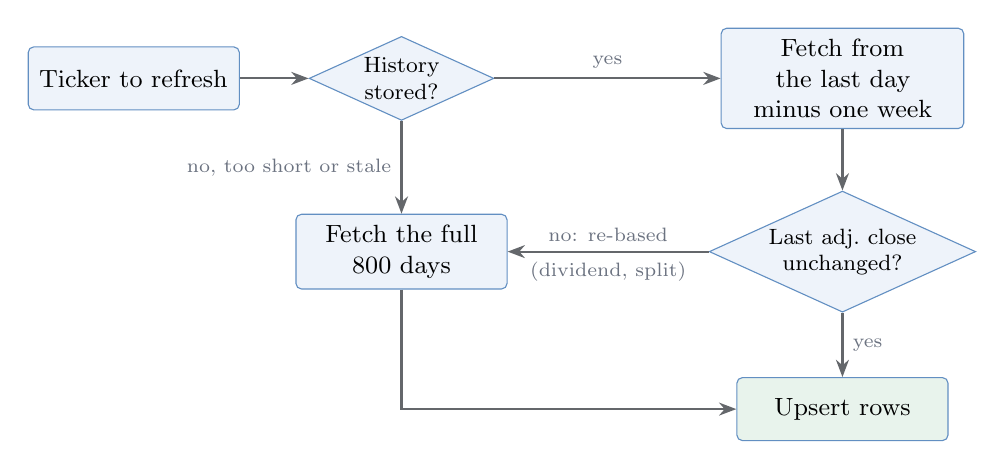
\begin{tikzpicture}[decision/.style={diamond, draw=accent!70, fill=boxfill, aspect=2.2, inner sep=1pt,
                                     font=\footnotesize, align=center}]
  \node[block=2.4cm] (start) at (0, 0)    {Ticker to refresh};
  \node[decision]    (have)  at (3.4, 0)  {History\\stored?};
  \node[block=2.8cm] (inc)   at (9.0, 0)  {Fetch from the last day\\minus one week};
  \node[decision]    (same)  at (9.0, -2.2) {Last adj.\ close\\unchanged?};
  \node[block=2.4cm] (full)  at (3.4, -2.2) {Fetch the full\\800 days};
  \node[block=2.4cm, fill=storefill] (store) at (9.0, -4.2) {Upsert rows};

  \draw[arr] (start) -- (have);
  \draw[arr] (have) -- node[lbl, above]{yes} (inc);
  \draw[arr] (have) -- node[lbl, left]{no, too short or stale} (full);
  \draw[arr] (inc) -- (same);
  \draw[arr] (same) -- node[lbl, right]{yes} (store);
  \draw[arr] (same.west) -- node[lbl, above]{no: re-based} node[lbl, below]{(dividend, split)} (full.east);
  \draw[arr] (full) |- (store);
\end{tikzpicture}
\caption{Incremental price refresh with a re-base check.}
\label{fig:refresh}
\end{figure}

It works: on the second daily run of the day, prices for 21 tickers came to 126 new rows instead of
about 11,000. Fundamentals use the same idea with filing dates.

The opposite problem is growth. At the end of every weekly screen a retention step deletes what no module
reads any more, using windows that match the longest look-back of the code that reads each table
(Table~\ref{tab:retention}). Passages cited by any suggestion are never deleted, so every citation keeps
working.

\begin{table}[htbp]
\centering\small
\begin{tabular}{@{}lll@{}}
\toprule
Data & Kept for & Longest reader \\
\midrule
Prices        & 800 days & Backfill window (the screen needs 420) \\
Fundamentals  & about 4 years of filings & 2-year analysis plus year-ago TTM figures \\
Macro         & 600 days & 500-day look-back plus release delays \\
News          & 400 days & Finnhub serves about a year \\
Filings       & 800 days & 2-year backfill \\
Logs          & 180 days & Debugging \\
\bottomrule
\end{tabular}
\caption{Retention windows. Stocks that drop out of the picks for 8 weeks also lose their documents;
they are backfilled again if they come back.}
\label{tab:retention}
\end{table}

\textbf{Gate.} Seven consecutive clean daily runs. The count restarted with the move to the local
database; the first clean runs were logged on 14 November.

% ==================================================================
\section{Phase 2: Knowledge}

\subsection{Numbers computed by code}

The quant engine (M4) is a set of pure functions over the stored data. As of any date it computes
trailing returns, moving averages, RSI \cite{wilder1978new}, MACD, volatility, drawdown, beta and
relative strength against SPY; point-in-time fundamentals rebuilt from the as-reported XBRL facts (TTM
revenue, margins, free cash flow, P/E, debt to equity); news-sentiment aggregates; and a macro snapshot
with release delays applied. The agent never computes any of this itself.

\subsection{Finding the right passages}

Retrieval (M5) is a retrieval-augmented generation setup in the sense of Lewis et al.\
\cite{lewis2020retrievalaugmented}; Gao et al.\ survey the wider family \cite{gao2023retrievalaugmented}.
Figure~\ref{fig:retrieval} shows the pipeline.

\begin{figure}[htbp]
\centering
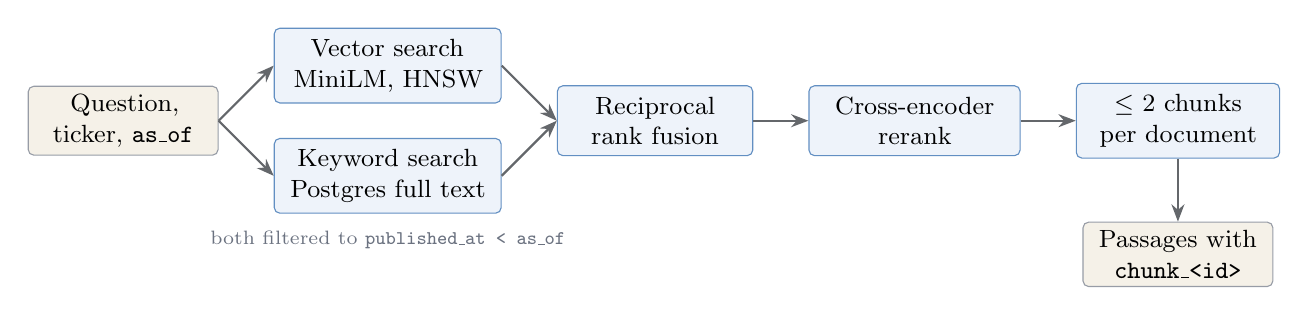
\begin{tikzpicture}[node distance=5mm and 7mm]
  \node[ext=2.2cm] (q) {Question,\\ticker, \code{as\_of}};
  \node[block=2.6cm, right=of q, yshift=7mm] (dense) {Vector search\\MiniLM, HNSW};
  \node[block=2.6cm, right=of q, yshift=-7mm] (kw) {Keyword search\\Postgres full text};
  \node[block=2.2cm, right=of dense, yshift=-7mm] (rrf) {Reciprocal\\rank fusion};
  \node[block=2.4cm, right=of rrf] (rr) {Cross-encoder\\rerank};
  \node[block=2.3cm, right=of rr] (div) {$\le$ 2 chunks\\per document};
  \node[ext=2.2cm, below=8mm of div] (out) {Passages with\\\code{chunk\_<id>}};

  \draw[arr] (q.east) -- (dense.west);
  \draw[arr] (q.east) -- (kw.west);
  \draw[arr] (dense.east) -- (rrf.west);
  \draw[arr] (kw.east) -- (rrf.west);
  \draw[arr] (rrf) -- (rr);
  \draw[arr] (rr) -- (div);
  \draw[arr] (div) -- (out);
  \node[lbl, below=1mm of kw] {both filtered to \code{published\_at < as\_of}};
\end{tikzpicture}
\caption{Hybrid retrieval. The two searches are fused without tuning, then reranked.}
\label{fig:retrieval}
\end{figure}

Dense search finds passages with similar meaning, in the style of dense passage retrieval
\cite{karpukhin2020dense}. Keyword search matters because exact terms carry a lot of meaning in finance:
tickers, product names, ``Item 1A''. The BEIR benchmark found that keyword retrieval is a strong baseline
that dense models often fail to beat on unfamiliar text \cite{thakur2021beir}. The two lists are merged
with reciprocal rank fusion \cite{cormack2009rrf}, which scores each chunk $d$ by
\begin{equation}
  \mathrm{RRF}(d) = \sum_{r \in \{\text{dense},\ \text{keyword}\}} \frac{1}{60 + \mathrm{rank}_r(d)},
\end{equation}
so it needs no tuning and ignores the different score scales of the two searches. A cross-encoder
trained on MS MARCO \cite{nogueira2019passage, bajaj2016marco} then re-scores the best candidates. Finally,
no document may fill more than two slots: Liu et al.\ found that models make less use of information buried
in the middle of a long context \cite{liu2023lost}, so fewer, more varied passages read better.

\textbf{Gate.} Ten test queries, each checked for the right ticker and source, nothing dated after
\code{as\_of}, and an expected keyword near the top. Hybrid search alone passed the automatic checks
but was on topic for only about 7 of 10 queries when I read the results; with the reranker it was 10 of
10, so the agent reranks by default. On the new database I repeated the check on five queries about this
week's picks (refining margins for VLO, medical cost trends for HUM, tariffs for ANF and others), and all
five came back with the right company's passages.

% ==================================================================
\section{The weekly screen}

Running search and the model on 900 stocks would take more than ten GPU-hours a week. So the pipeline
works in two stages (Figure~\ref{fig:funnel}): screen everything cheaply with prices and SEC data, then
spend the expensive steps on the top twenty.

\begin{figure}[htbp]
\centering
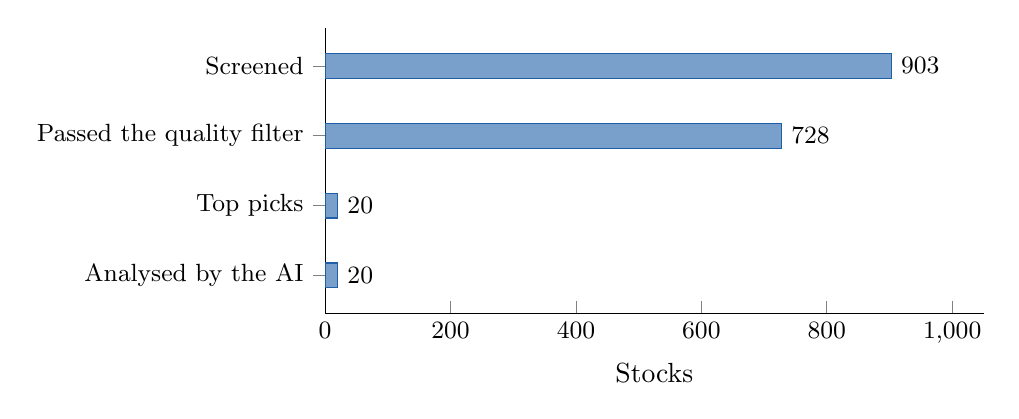
\begin{tikzpicture}
\begin{axis}[
  xbar, width=0.82\linewidth, height=5.2cm,
  xmin=0, xmax=1050, xlabel={Stocks},
  symbolic y coords={Analysed by the AI, Top picks, Passed the quality filter, Screened},
  ytick=data, y tick label style={font=\small}, x tick label style={font=\small},
  bar width=9pt, enlarge y limits=0.18,
  nodes near coords, nodes near coords style={font=\small},
  axis x line*=bottom, axis y line*=left,
]
\addplot[fill=accent!60, draw=accent] coordinates {
  (903,Screened) (728,Passed the quality filter) (20,Top picks) (20,Analysed by the AI)};
\end{axis}
\end{tikzpicture}
\caption{The two-stage funnel in the screen of 15 November 2026 (as of the 14 November close).}
\label{fig:funnel}
\end{figure}

The universe is the S\&P 500 plus the S\&P MidCap 400. The quality filter keeps companies whose latest
quarter ended less than 200 days ago, with positive trailing net margin and positive free cash flow, in
the spirit of the profitability literature \cite{novymarx2013other}. Among the companies that pass, the
score is
\begin{equation}
  S = 0.50\, z(r_{12-1}) + 0.25\, z(r^{\text{rel}}_{6\text{m}}) + 0.25\, z(r^{\text{rel}}_{3\text{m}}) - 0.20\, z(\sigma_{6\text{m}}),
\end{equation}
where $r_{12-1}$ is the classic twelve-minus-one-month momentum return \cite{jegadeesh1993returns},
the relative returns are measured against SPY, $\sigma_{6\text{m}}$ is six-month volatility, and each
$z$-score is clipped at $\pm 3$. The top twenty become the picks; a pick with no documents yet gets two
years of news and filings, which are then chunked, embedded and scored.

The screen replaced a hand-picked watchlist. Until 12 November the app followed five large technology
stocks chosen by hand (Figure~\ref{fig:earlyglance}); the first screened week put twenty quite different
companies in their place (Figure~\ref{fig:appglance} in Section~\ref{sec:readers}).

\screenshot[0.95]{early-glance.png}{The app before the screen existed: a fixed watchlist of five stocks,
run of 12 November.}{fig:earlyglance}

This week the picks leaned heavily towards health care and energy (Figure~\ref{fig:sectors}). That is
what momentum does: it follows whatever has been working, which is worth keeping in mind when reading the
views.

\begin{figure}[htbp]
\centering
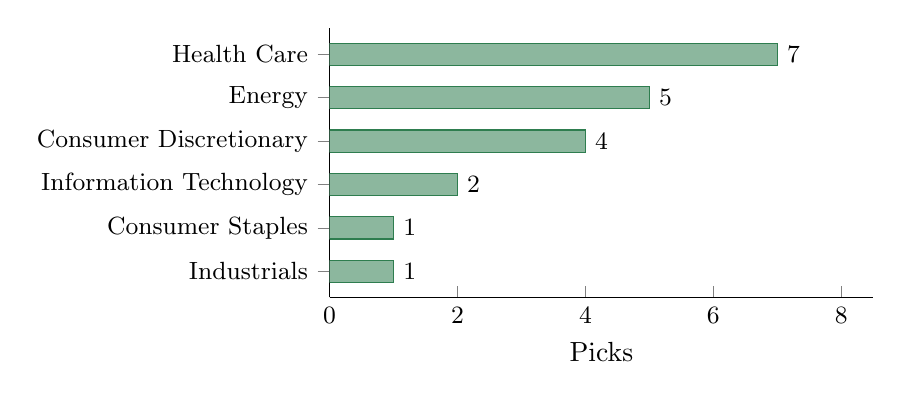
\begin{tikzpicture}
\begin{axis}[
  xbar, width=0.7\linewidth, height=5cm, xmin=0, xmax=8.5, xlabel={Picks},
  symbolic y coords={Industrials, Consumer Staples, Information Technology, Consumer Discretionary, Energy, Health Care},
  ytick=data, y tick label style={font=\small}, x tick label style={font=\small}, xtick={0,2,...,8},
  bar width=8pt, enlarge y limits=0.12, nodes near coords, nodes near coords style={font=\small},
  axis x line*=bottom, axis y line*=left,
]
\addplot[fill=good!55, draw=good] coordinates {
  (1,Industrials) (1,Consumer Staples) (2,Information Technology) (4,Consumer Discretionary) (5,Energy) (7,Health Care)};
\end{axis}
\end{tikzpicture}
\caption{Sectors of the twenty picks.}
\label{fig:sectors}
\end{figure}

% ==================================================================
\section{Phase 3: The agent}

\subsection{How it works}

For each pick, the agent (M6) works in a loop: it reasons, calls a tool, reads the result and repeats
until it has saved both views (Figure~\ref{fig:agent}). This is the ReAct pattern
\cite{yao2022react}, with tool use in the spirit of Toolformer \cite{schick2023toolformer}. The model is
Qwen3.5~4B, a text-only build that fits a 6\,GB laptop GPU, with ``thinking'' switched on; the Qwen3
report describes the combined thinking and non-thinking design \cite{yang2025qwen3}.

\begin{figure}[htbp]
\centering
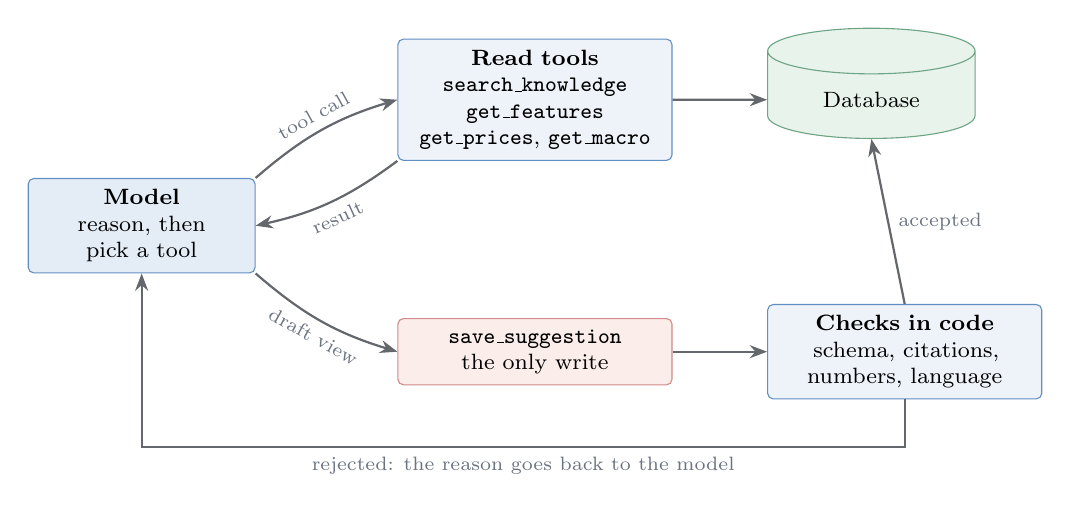
\begin{tikzpicture}[node distance=7mm and 9mm, block/.append style={font=\footnotesize},
                    store/.append style={font=\footnotesize}]
  \node[block=2.6cm, fill=accent!12] (llm) {\textbf{Model}\\reason, then\\pick a tool};
  \node[block=3.2cm, right=18mm of llm, yshift=16mm] (read) {\textbf{Read tools}\\\code{search\_knowledge}\\\code{get\_features}\\\code{get\_prices}, \code{get\_macro}};
  \node[block=3.2cm, right=18mm of llm, yshift=-16mm, fill=warnfill, draw=bad!60] (save) {\textbf{\code{save\_suggestion}}\\the only write};
  \node[block=3.2cm, right=12mm of save] (checks) {\textbf{Checks in code}\\schema, citations,\\numbers, language};
  \node[store=2.4cm, right=12mm of read] (db) {Database};

  \draw[arr] (llm.north east) to[bend left=12] node[lbl, above, sloped]{tool call} (read.west);
  \draw[arr] (read.south west) to[bend left=12] node[lbl, below, sloped]{result} (llm.east);
  \draw[arr] (read) -- (db);
  \draw[arr] (llm.south east) to[bend right=12] node[lbl, below, sloped]{draft view} (save.west);
  \draw[arr] (save) -- (checks);
  \draw[arr] (checks.south) -- ++(0,-6mm) -| node[lbl, below, pos=0.25]{rejected: the reason goes back to the model} (llm.south);
  \draw[arr] (checks.north) -- node[lbl, right]{accepted} (db.south);
\end{tikzpicture}
\caption{The agent loop. Each pick gets at most 16 model turns and 16 tool calls, plus one retry.}
\label{fig:agent}
\end{figure}

\subsection{Guardrails that live in code}

A 4B model doesn't reliably follow rules written in a prompt, so the important ones are enforced where
the model can't argue with them:

\begin{itemize}
  \item \textbf{Ticker and date are fixed by code.} No tool takes an \code{as\_of} argument, and the saved
        ticker and date are filled in by the system.
  \item \textbf{Citations must have been seen.} Every \code{chunk\_<id>} in a view must have come back from
        a search in the same conversation, which applies the idea of checked citations
        \cite{gao2023enabling} at the moment of saving.
  \item \textbf{Numbers must come from tools.} Every figure that looks like a claim (a decimal, a
        percentage, an amount) has to match, after rounding, a value some tool returned.
  \item \textbf{Stances are relative.} Bullish means the model expects the stock to beat SPY over the
        horizon, which is how the evaluation will score it.
\end{itemize}

\subsection{The first run on the local database}

The run of 14 November finished with status \emph{ok}: all twenty picks got both views, forty
suggestions in 32 minutes. Four picks needed their one retry, two because Ollama returned an internal
error and two because they hit the tool-call cap.

The guardrails were busy. Of 89 attempts to save a view, 49 were rejected and sent back with the reason:
26 because a number didn't match any tool output, and 23 because a required field was missing. In every
case the model fixed the problem on a later turn. I find this the most reassuring number in the run,
because each of those 26 would otherwise have been a confident, plausible and unsupported figure.

\begin{figure}[htbp]
\centering
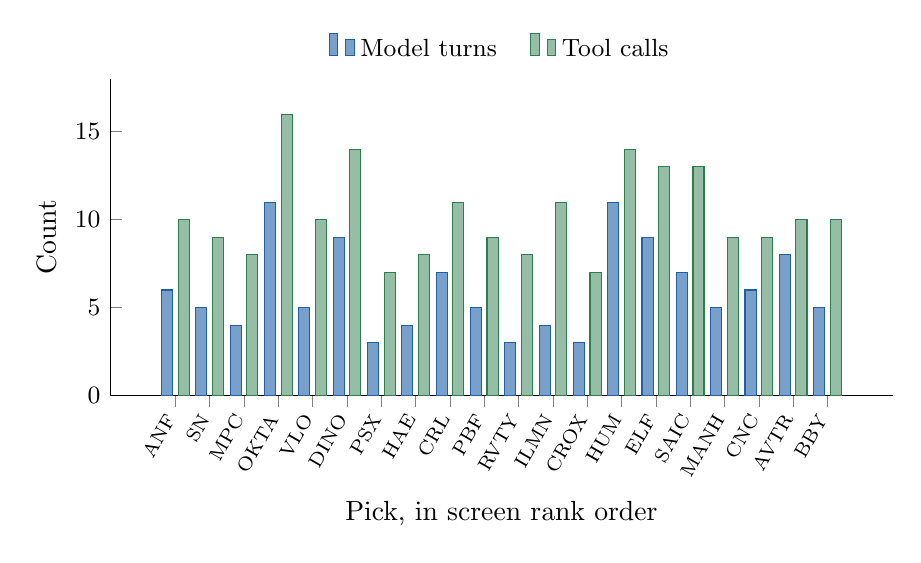
\begin{tikzpicture}
\begin{axis}[
  ybar, width=0.95\linewidth, height=5.6cm, ymin=0, ymax=18,
  ylabel={Count}, xlabel={Pick, in screen rank order},
  symbolic x coords={ANF,SN,MPC,OKTA,VLO,DINO,PSX,HAE,CRL,PBF,RVTY,ILMN,CROX,HUM,ELF,SAIC,MANH,CNC,AVTR,BBY},
  xtick=data, x tick label style={rotate=60, anchor=east, font=\scriptsize}, y tick label style={font=\small},
  bar width=4pt, legend columns=2, legend style={font=\small, at={(0.5,1.02)}, anchor=south, draw=none,
    /tikz/every even column/.append style={column sep=10pt}},
  axis x line*=bottom, axis y line*=left,
]
\addplot[fill=accent!60, draw=accent] coordinates {
  (ANF,6) (SN,5) (MPC,4) (OKTA,11) (VLO,5) (DINO,9) (PSX,3) (HAE,4) (CRL,7) (PBF,5)
  (RVTY,3) (ILMN,4) (CROX,3) (HUM,11) (ELF,9) (SAIC,7) (MANH,5) (CNC,6) (AVTR,8) (BBY,5)};
\addplot[fill=good!50, draw=good] coordinates {
  (ANF,10) (SN,9) (MPC,8) (OKTA,16) (VLO,10) (DINO,14) (PSX,7) (HAE,8) (CRL,11) (PBF,9)
  (RVTY,8) (ILMN,11) (CROX,7) (HUM,14) (ELF,13) (SAIC,13) (MANH,9) (CNC,9) (AVTR,10) (BBY,10)};
\legend{Model turns, Tool calls}
\end{axis}
\end{tikzpicture}
\caption{Effort per pick in the final attempt. OKTA and HUM needed the most work; the simplest picks were
done in three turns.}
\label{fig:effort}
\end{figure}

The views themselves lean bullish, especially over one to three months (Figure~\ref{fig:stances}).
That is partly the screen at work, since the picks were chosen for strong momentum, and partly a known
tendency of language models to be agreeable. Confidence stayed in a narrow band, 0.55 to 0.62 with a mean
of 0.59, as the prompt asks. Whether those numbers mean anything is exactly what the evaluation phase has
to establish \cite{guo2017calibration}.

\begin{figure}[htbp]
\centering
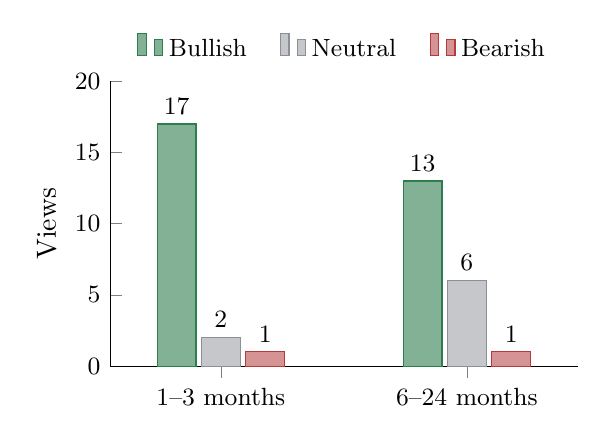
\begin{tikzpicture}
\begin{axis}[
  ybar, width=0.62\linewidth, height=5.2cm, ymin=0, ymax=20, ylabel={Views},
  symbolic x coords={1--3 months, 6--24 months}, xtick=data, enlarge x limits=0.45,
  bar width=14pt, nodes near coords, nodes near coords style={font=\small},
  legend style={font=\small, at={(0.5,1.03)}, anchor=south, legend columns=3, draw=none,
    /tikz/every even column/.append style={column sep=10pt}},
  axis x line*=bottom, axis y line*=left, x tick label style={font=\small}, y tick label style={font=\small},
]
\addplot[fill=good!60, draw=good] coordinates {(1--3 months,17) (6--24 months,13)};
\addplot[fill=neutral!50, draw=neutral] coordinates {(1--3 months,2) (6--24 months,6)};
\addplot[fill=bad!55, draw=bad] coordinates {(1--3 months,1) (6--24 months,1)};
\legend{Bullish, Neutral, Bearish}
\end{axis}
\end{tikzpicture}
\caption{Stances of the forty views. The long horizon is noticeably more cautious.}
\label{fig:stances}
\end{figure}

\subsection{The same run without search}

To find out what the documents actually contribute, the agent runs a second time each week on the same
picks with the search tool taken away and citations switched off. Everything else stays the same: the
model, the prompt, the features and the limits. These views are stored next to the real ones but never
published, and the evaluation scores both (Section~\ref{sec:eval}).

\begin{table}[htbp]
\centering\small
\caption{The full system and the no-retrieval variant on the same twenty picks, week of 14 November 2026.}
\label{tab:ablation}
\begin{tabular}{@{}lrr@{}}
\toprule
 & Full & No retrieval \\
\midrule
Run status, views saved & ok, 40 & ok, 40 \\
Wall-clock time & 32 min & 31 min \\
Save attempts rejected & 49 of 89 & 73 of 113 \\
\quad of which unmatched numbers & 26 & 71 \\
\quad of which period labels only (``3m'') & 13 & 51 \\
\quad of which missing or invalid fields & 23 & 2 \\
Citations & 152 & 0 \\
1--3 months: bullish / neutral / bearish & 17 / 2 / 1 & 14 / 6 / 0 \\
6--24 months: bullish / neutral / bearish & 13 / 6 / 1 & 12 / 6 / 2 \\
Mean confidence & 0.59 & 0.59 \\
\midrule
Same stance, 1--3 months & \multicolumn{2}{c}{13 of 20, $\kappa = 0.07$} \\
Same stance, 6--24 months & \multicolumn{2}{c}{13 of 20, $\kappa = 0.32$} \\
\bottomrule
\end{tabular}
\end{table}

Both versions finished every stock, and they agreed on thirteen of twenty stances at each horizon
(Table~\ref{tab:ablation}). Once agreement by chance is removed, the picture is clearer: over one to three
months the two barely agree ($\kappa = 0.07$), while over six to twenty-four months they agree fairly
($\kappa = 0.32$). The documents mostly move the short-term call, which is where news should matter. Which
version is closer to what the market does is still unknown.

The log of rejections showed something I hadn't expected. The number check reads ``3m'' as three million,
but the model means three months, as in ``3m momentum''. Without documents to quote, the model talks about
momentum more, and 51 of its 71 rejected numbers were labels like this. It cost turns but no views. Fixing
it changes a guardrail in the middle of an experiment, so the fix went in straight after the first week and
is recorded as an amendment: a whole number up to 60 written directly against ``m'' with no dollar sign now
counts as months, while ``\$3m'', ``3.5m'' or ``250m'' are still checked as millions.

\textbf{Gate.} Four weekly runs in which every view is valid and cited. The earlier runs were on the hosted
database and weren't copied over, so the count stands at one of four.

% ==================================================================
\section{Phase 4: Getting results to readers}

\subsection{Why the app reads a file, not a server}

The app is a single Flutter codebase for the web, Android and iOS, and its web build is published on
GitHub Pages. GitHub Pages serves only static files, and the data lives in a database on my laptop, which
nothing on the internet can reach. The obvious fix is a tunnel that exposes a small API, and I built one,
but it needs a domain and only works while the laptop is on.

The approach I kept is simpler. After every run, the laptop exports exactly what the app shows into one
file: this week's picks, the views (and last week's, to mark what changed), a year of prices and the cited
passages. The file is encrypted, pushed to the repository and published beside the app
(Figure~\ref{fig:publish}). The app downloads it and decrypts it in the browser. Nothing runs online, and
the app keeps working while the laptop is off; it is as fresh as the last push.

\begin{figure}[htbp]
\centering
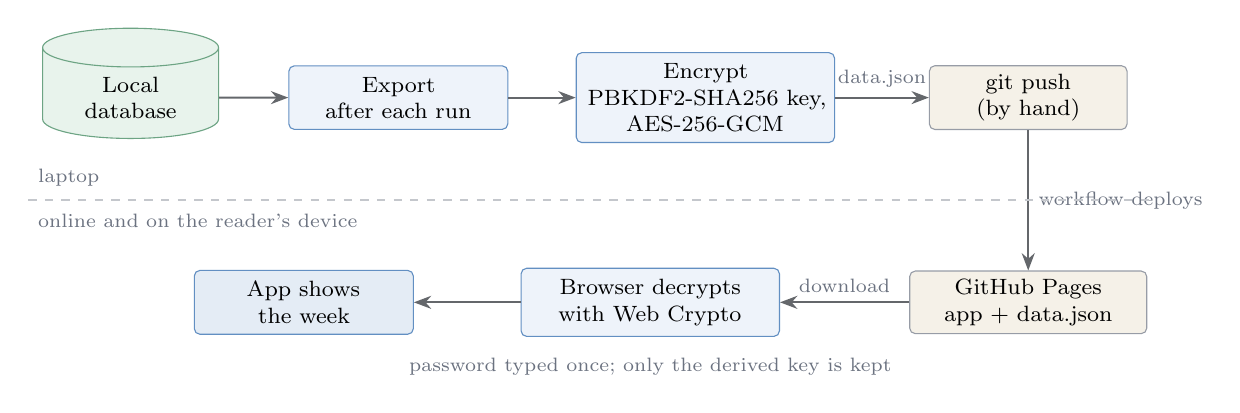
\begin{tikzpicture}[block/.append style={font=\footnotesize}, ext/.append style={font=\footnotesize},
                    store/.append style={font=\footnotesize}]
  % top row: on the laptop
  \node[store=2.0cm]  (db)    at (0, 0)      {Local\\database};
  \node[block=2.5cm]  (exp)   at (3.4, 0)    {Export\\after each run};
  \node[block=3.0cm]  (enc)   at (7.3, 0)    {Encrypt\\PBKDF2-SHA256 key,\\AES-256-GCM};
  \node[ext=2.3cm]    (repo)  at (11.4, 0)   {git push\\(by hand)};
  % bottom row: online and on the reader's device
  \node[ext=2.8cm]    (pages) at (11.4, -2.6) {GitHub Pages\\app + data.json};
  \node[block=3.0cm]  (dec)   at (6.6, -2.6)  {Browser decrypts\\with Web Crypto};
  \node[block=2.5cm, fill=accent!12] (app) at (2.2, -2.6) {App shows\\the week};

  \draw[arr] (db) -- (exp);
  \draw[arr] (exp) -- (enc);
  \draw[arr] (enc) -- node[lbl, above]{data.json} (repo);
  \draw[arr] (repo) -- node[lbl, right]{workflow deploys} (pages);
  \draw[arr] (pages) -- node[lbl, above]{download} (dec);
  \draw[arr] (dec) -- (app);
  \node[lbl, below=1.5mm of dec] {password typed once; only the derived key is kept};
  \draw[muted!40, dashed] (-1.3, -1.3) -- (13.0, -1.3);
  \node[lbl, anchor=south west] at (-1.3, -1.25) {laptop};
  \node[lbl, anchor=north west] at (-1.3, -1.35) {online and on the reader's device};
\end{tikzpicture}
\caption{Publishing without a server. The file is public but unreadable without the password.}
\label{fig:publish}
\end{figure}

\subsection{How the file is protected}

The key is derived from a password with PBKDF2-SHA256 \cite{rfc8018} (250,000 iterations and a random
16-byte salt), and the data is encrypted with AES-256 in Galois/Counter Mode \cite{nist80038d}, which also
detects any change to the file. Every export uses a fresh 12-byte nonce. Two details make it pleasant to
use:

\begin{itemize}
  \item The salt stays the same while the password does, so a device that unlocked once keeps opening
        straight away. Only the derived key is stored on the device, never the password.
  \item If nothing changed since the last export, the file isn't rewritten, so there is nothing to push.
\end{itemize}

The honest weak point is that anyone can download the file and try passwords offline. The default
password is therefore 24 random characters, about 144 bits, far beyond guessing. The same file was
decrypted by the Python exporter's tests, by the Dart test suite and by Web Crypto in Node.js, which is
the same interface the browser uses.

Pushing the file starts the same GitHub Actions workflow that builds the app
(Figure~\ref{fig:ci}): it runs the Flutter tests, builds the web version and an Android APK, puts the data
file next to the web build and deploys it.

\screenshot[0.62]{ci-workflow.png}{The publishing workflow on GitHub Actions: tests, the web and Android
builds, then the deploy to GitHub Pages.}{fig:ci}

\subsection{What a reader sees}\label{sec:readers}

The first visit asks for the password (Figure~\ref{fig:unlock}). After that the app opens on this week's
research: how many stocks were screened, how many views there are and how many changed since last week
(Figure~\ref{fig:apphome}), followed by a grid of all twenty picks with their rank, momentum and both
stances (Figure~\ref{fig:appglance}). Each pick then has its own scene with the thesis, bull and bear case,
valuation, catalysts and risks, each with its sources, and a page with a twelve-month chart against SPY
and the history of earlier views (Figure~\ref{fig:tickerchart}). Since the first run each ticker also carries
its company name, on the glance cards, in the scenes, in the Compare table and in the ticker page title, so
readers don't need to know that DINO is HF Sinclair. Names come from the index lists; SEC's upper-case
registrant names (``ABERCROMBIE \& FITCH CO /DE/'') only fill gaps and are tidied for display. The
screenshots were taken before names were added.

\screenshot[0.8]{app-unlock.png}{The unlock screen on GitHub Pages. The password never leaves the
device.}{fig:unlock}
\screenshot[0.85]{app-home.png}{The opening screen after the first run on the local database: 903 stocks
screened, 20 picks, 40 views and 130 cited passages.}{fig:apphome}
\screenshot[0.95]{app-glance.png}{All twenty picks at a glance, in screen rank order, with their momentum
and both stances.}{fig:appglance}
\screenshot[0.95]{ticker-chart.png}{A ticker page: the stock against SPY over twelve months, both indexed
to 100, followed by its earlier views. This one is from the run of 12 November, when the app still followed
a fixed watchlist.}{fig:tickerchart}

\subsection{The other two outputs}

A Telegram bot sends a short digest after each weekly run, or an alert if it failed. A Django dashboard,
used only on the laptop, shows the same views with their cited passages, the computed features the agent
saw, and the status of every pipeline run.

% ==================================================================
\section{Running it every week}

Four Windows scheduled tasks run the pipeline (Table~\ref{tab:schedule}). Each script starts Docker and
the database if needed, shows its progress live in the terminal (each step with a counter, a progress bar
and its time), writes the details to a log file and finishes by exporting the app's data.

\begin{table}[htbp]
\centering\small
\begin{tabularx}{\linewidth}{@{}l l X@{}}
\toprule
Task & When (local time) & Does \\
\midrule
Daily refresh & Weekdays 23:45 & New prices, news, filings, fundamentals, macro; chunk, embed, score \\
Weekly screen & Saturday 01:30 & Screen $\sim$900 stocks, backfill new picks, retention \\
Weekly AI run & Saturday 09:00 & Views for the twenty picks, Telegram digest \\
Weekly baseline & Saturday 10:30 & The same picks without search, for the evaluation; not published \\
\bottomrule
\end{tabularx}
\caption{The schedule. A run missed because the laptop was off starts when it is next on.}
\label{tab:schedule}
\end{table}

Figure~\ref{fig:timeline} shows what the first full day on the local database actually looked like.

\begin{figure}[htbp]
\centering
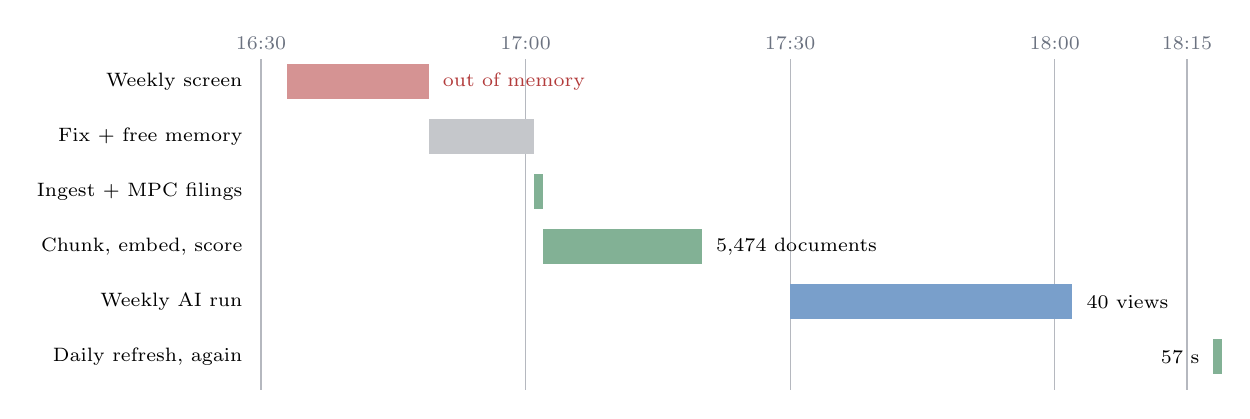
\begin{tikzpicture}[x=0.112cm, y=7mm]
  % time axis: minutes after 16:30
  \foreach \t/\l in {0/16:30, 30/17:00, 60/17:30, 90/18:00, 105/18:15} {
    \draw[muted!50] (\t,0.4) -- (\t,-5.6);
    \node[lbl, above] at (\t,0.4) {\l};
  }
  \newcommand{\ganttbar}[5]{% row, start, end, colour, label
    \fill[#4] (#2,-#1-0.32) rectangle (#3,-#1+0.32);
    \node[font=\scriptsize, anchor=east] at (-1,-#1) {#5};}
  \ganttbar{0}{3}{19}{bad!55}{Weekly screen}
  \ganttbar{1}{19}{31}{neutral!50}{Fix + free memory}
  \ganttbar{2}{31}{32}{good!60}{Ingest + MPC filings}
  \ganttbar{3}{32}{50}{good!60}{Chunk, embed, score}
  \ganttbar{4}{60}{92}{accent!60}{Weekly AI run}
  \ganttbar{5}{108}{109}{good!60}{Daily refresh, again}
  \node[font=\scriptsize, text=bad, anchor=west] at (19.5,0) {out of memory};
  \node[font=\scriptsize, anchor=west] at (50.5,-3) {5{,}474 documents};
  \node[font=\scriptsize, anchor=west] at (92.5,-4) {40 views};
  \node[font=\scriptsize, anchor=east] at (107.5,-5) {57 s};
\end{tikzpicture}
\caption{The first full run, 14 November 2026. The screen crashed while embedding, the fix took ten minutes,
and everything after that ran cleanly.}
\label{fig:timeline}
\end{figure}

% ==================================================================
\section{What went wrong, and what I learned}

The code worked the first time more often than the machine did. Almost every failure in the first full run
came down to memory, on a laptop with 16\,GB of RAM and a 12\,GB page file shared with an editor, a browser,
Docker and a MySQL server.

\begin{itemize}
  \item \textbf{Embedding crashed the screen.} With 1.4\,GB of commit memory free, loading the embedding model
        failed with ``the paging file is too small''. Worse, processing marked six documents as permanently
        failed, so they would never have been retried. Processing now stops on an out-of-memory error and
        leaves the documents queued.
  \item \textbf{One SEC filing was too big to download.} A single document from Marathon Petroleum was read
        into memory in one piece and raised a \code{MemoryError}. Downloads now stream and stop at 25\,MB,
        which is far more than the 300,000 characters of text that are kept anyway.
  \item \textbf{Ollama held on to the model.} After the AI run finished, Ollama kept the model loaded for
        another half hour, about 6\,GB, and the next job couldn't even import its maths library. The weekly
        run now unloads the model as soon as it is done.
  \item \textbf{Windows text encoding.} When output went to a file, as it does in scheduled tasks, Windows
        used a code page that couldn't print the progress symbols, and the run crashed on its first line. It
        now falls back to plain ASCII marks.
\end{itemize}

The general lesson is that on a personal machine the environment is part of the system. A pipeline that
only works when the owner remembers to close the browser isn't finished.

% ==================================================================
\section{Limitations and what comes next}

\subsection{Known limitations}

\begin{itemize}
  \item Finnhub's free tier gives only headlines and summaries, and about a year of them.
  \item Long 10-K filings are cut at 300,000 characters, so the end of a very long filing can be lost.
  \item The universe is today's index membership, so any backtest suffers from survivorship bias.
  \item Even with every input dated correctly, the model's own training data can contain hindsight
        \cite{glasserman2023assessing}. Backtests before its training cutoff should be read as optimistic.
  \item A small model sometimes puts a real number under the wrong label; the number check can't catch that.
  \item One week of views is not evidence of anything yet. The primary evaluation needs twelve closed weeks.
\end{itemize}

\subsection{Phase 5: evaluation}\label{sec:eval}

The evaluation module is built and runs after every weekly screen. It scores each view once its window has
closed: the stock's return minus SPY's, from the first trading day after the view to 21, 63 and 252 trading
days later, on adjusted prices. A bullish view is right if the stock beat SPY and a bearish one if it
trailed; neutral views have no direction and are left out of the hit rate. The same scoring is applied to
four comparators, so the agent can be told apart from the screen it starts from: the screen's twenty picks
treated as bullish, a random sample of quality stocks of the same size (seeded by the date so it can be
repeated), all quality stocks, and the agent without search. The report gives hit rates with a binomial
test, the excess return of bullish minus bearish views with confidence intervals that resample whole weeks,
calibration of the stated confidence \cite{guo2017calibration}, and whether claims match their cited
passages, judged by two annotators with Cohen's $\kappa$.

The rules were written down before any result existed. The main test is the one-to-three-month views at 63
trading days, and it waits for twelve closed weeks, around May 2027. Until then the report says
``preliminary'' at the top.

\subsection{Phase 5: quantum}

One more piece of research is planned. It turns the views into portfolio weights and compares a
classical mean-variance optimiser with the Quantum Approximate Optimization Algorithm
\cite{farhi2014quantum} on a simulator, following Brandhofer et al.'s benchmark of QAOA for portfolio
optimisation \cite{brandhofer2022benchmarking}; a quantum-kernel regime classifier
\cite{havlicek2018supervised} is a possible second experiment.

% ==================================================================
\section{Conclusion}

A free, 4-billion-parameter model on a laptop can produce structured, cited stock research, as long as the
system around it does the parts the model is bad at. Code fixes the date and the ticker, computes every
number, checks every citation and rejects anything that doesn't hold up; in the first local run it
rejected more than half of the model's attempts to save, and the model corrected every one. The rest of
the work was ordinary engineering: storing data with the moment it became public, fetching only what
changed, deleting what nothing reads, and getting results to readers without running a server. Whether
the views are any good is a question for the evaluation phase, and that is the right order to ask it in.

\appendix
\section{Reproducing it}

\begin{lstlisting}
.\scripts\setup.ps1                     # venv, packages, .env, Ollama model
docker compose up -d                    # PostgreSQL 17 + pgvector, 127.0.0.1:5433
.venv\Scripts\python -m common.db_init  # create the schema
run_screen.cmd                          # first screen and backfill (1.5-2 h)
run_daily.cmd --days 730                # two-year backfill for the picks
run_weekly.cmd                          # the AI run (about 30 min)
.\scripts\register_tasks.ps1            # the three scheduled tasks
\end{lstlisting}

After a run, push \code{site-data/data.json} to publish the new data to the app.

\section{Data in the store after the first run}

\begin{table}[H]
\centering\small
\begin{tabular}{@{}lr@{}}
\toprule
Data & Rows \\
\midrule
Daily prices                & 495,468 \\
SEC financial facts         & 429,924 \\
News items (scored by FinBERT) & 4,875 \\
SEC filings                 & 600 \\
Searchable passages         & 37,879 \\
Macro observations          & 428 \\
Agent tool calls            & 253 \\
Suggestions                 & 40 \\
\bottomrule
\end{tabular}
\caption{Row counts on 14 November 2026.}
\end{table}

\printbibliography[heading=bibintoc, title={References}]

\end{document}
